\documentclass[11pt]{article}
\usepackage{amssymb}
\usepackage[english]{babel}
\usepackage{fullpage}
\usepackage{multirow}
\usepackage{graphicx}
\usepackage{sidecap}
\usepackage{caption}
%\usepackage{subcaption}

\usepackage[utf8]{inputenc}

\usepackage{color}

\makeatletter

\newcommand{\rem}[1]{\fbox{\sf {#1}}}

\title{LOG8415 \\ Concepts avanc\'{e}s en infonuagique \\ TP1}

\author{
	Antoine Delaite, Mohamed Amine Barrak et Philippe Troclet \\
		\\
	Travail pr\'{e}sent\'{e} \`a \\
		\\
	Foutse Khomh et S. Amirhossein Abtahizadeh \\
		\\
	D\'{e}partement G\'{e}nie Informatique et G\'{e}nie Logiciel \\
	\'{E}cole Polytechnique de Montr\'{e}al, Qu\'{e}bec, Canada
}

\date{28 Janvier 2017}

\begin{document}
\maketitle

\section{Introduction}
%The goal of this paper is to find a solution for the online retailer company
%(Alpha X) to migrate to the Cloud Computing (Azure and Amazon). The
%architecture of the elements of the society are presented in Figure 1.For this
%purpose, we compare the performance of Amazon Web Services (AWS) and Azure
%virtual machines (VM) in terms of several criteria such CPU computing ,memory
%access , disk I/O, Input/Output operations Per Second (IOPS) and network speed.
%AWS is a cloud-computing platform offered by Amazon while Azure is offered by
%Microsoft. We realize different benchmarks of Azure and AWS instances in order
%to study their performances and subsequently affect the best instances with
%regard to disk speed, storage capacity, IO speed and cost.

Le présent document vise à exhiber une stratégie appropriée pour la migration de la compagnie \textit{Alpha X} vers les services du \textit{cloud}. L'architecture désirée est visible ci-dessous. Afin d'identifier les meilleures instances pour chaque type VM (calcul, stockage, etc), nous mettons en place plusieurs \textit{benchmark}. Chacun testera une capacité essentielle des machines. Ainsi, la capacité de calcul, le débit d'écriture (IO), le nombre d'opérations d'IO par seconde (IOPS) et la performance du réseau seront évalués. Ainsi, de ces tests, nous pourrons extraire quelle instance de quel fournisseur répond le mieux aux critères.
~\\
\centerline{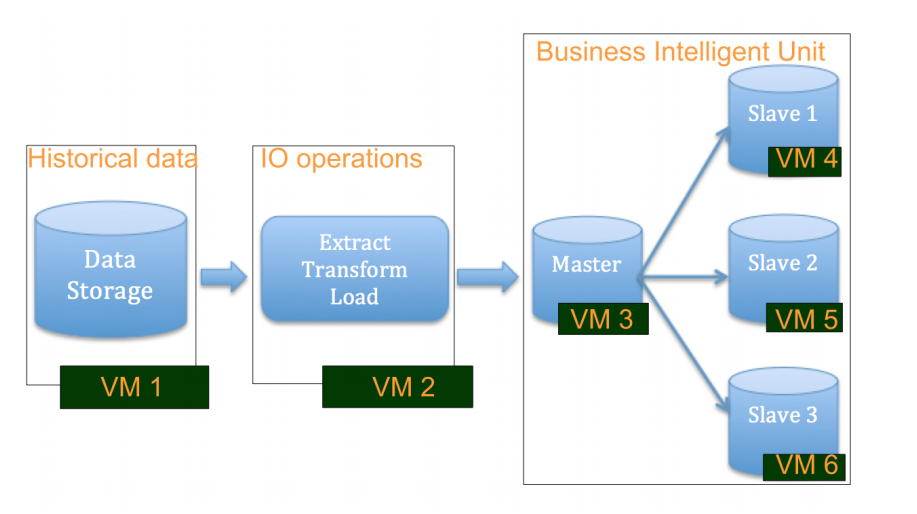
\includegraphics[width=0.75\textwidth]{images/design_architechture_element}} % Include the image placeholder.png
\centerline{Figure 1: Design Architecture Elements} 
~\\

\section{Caractéristiques des différentes machines}

Pour tester les configurations des machines localement,
nous avons utilisé les commandes standards UNIX suivantes:
\begin{itemize}
	\item Pour le nombres de coeurs: nproc
	\item Pour la taille de la RAM: free -h
	\item Pour la taille du disque: df -h /
\end{itemize}
On note que la taille du disque que nous avons est celle que l'on
peut accéder facilement, soit la taille du répertoire home. Nous
avons noté que sur Amazon la moitié du disque était consacrée à
/dev, tandis que sur Azure la mémoire est en général découpée en
30G pour l'utilisateur plus une partition contenant le reste.
On a donc assez peu d'espace disque sur les instances d'Amazon EC2.
Les caractéristiques correspondent bien avec celles annoncées sur 
les sites respectifs d'Amazon et d'Azure. \\

\begin{tabular} {  p{2.3cm}  p{2.8cm} || c  c  c  c   }
	\multicolumn{6} {c} {Table 2.1: VM Instances} \\
	\hline  \hline
	Cloud Service & Instance Type & CPU & Memory & Disk & Networking Performance \\
		      & & (CU) & (GiB) & (GB) & bandwidth\\
	\hline \hline
	\multirow{3}{*}{AWS} &  t2.small  & 1 & 2 & 9.2 & Low to Moderate \\
			     & m4.2xlarge  & 8 & 32 & 9.2 & High \\
	       & c4.4xlarge  & 16 & 30 & 9.2 & High \\
	\hline  \hline
	\multirow{3}{*}{Azure} & A1  & 1 & 1.6G & 29 & Moderate \\
			       &  A8 v2 & 8 & 16 & 80 & High \\
		 &  D5 v2 & 16 & 56 & 800 & Extremely High \\
	\hline  \hline
\end{tabular}\\

On notera que les 800GB indiqués dans le cas de l'instance D5 ne représentent pas un espace de stockage que l'utilisateur peut utiliser pour sauvegarder ses données définitivement. Il s'agit d'un espace de stockage temporaire où les données ne sont pas destinées à rester. Pour la sauvegarde des données, l'utilisateur doit utiliser les 30GB qui lui sont attribués.
%%\begin{center}
%%\begin{tabular}{|c | c | c | c|c|}
%%	MACHINE & COEURS & RAM & DISQUE & RESEAU \\
%%	\hline
%%	t2.small & 1 & 2G & 9.2G & \\
%%	\hline
%%	m4.2xlarge& 8 & 31G & 9.2G & \\
%%	\hline
%%	c4.4xlarge & 16 & 29G & 9.2G&\\
%%	\hline
%%	A1 & 1 & 1.6G & 29G & \\
%%	\hline
%%	A8 & 8 & 16G& 29G &\\
%%	\hline
%%	D5\_v2 & 16 & 55G & 29G &\\
%%\end{tabular}
%%\end{center}

\section{Méthode de benchmarking}

Afin de tester les capacités des instances d'Amazon EC2 et Azure de Microsoft,
nous avons développé plusieurs scripts. Un script lançant une connexion ssh et
lançant les commandes à distance. Ensuite deux autres programmes utilisant les
API d'Azure et d'Amazon respectivement créant des machines et les supprimant,
et appelant le script principal pour benchmarker les instances.\\
Il est pertinent de souligner que les scripts présentés ci-dessus peuvent être appelés depuis d'autres scripts pour réaliser un enchaînement précis d'opérations.
\subsection{bench.sh}
bench.sh est notre script principal qui prend en argument un nom de test et une
machine et qui lance le test sur la machine. Il collecte ensuite le log
résultant et le copie sur la machine locale. Ce script est écrit en bash et se
trouve dans le dossier benchmark/. \\
Chaque test est décomposé en deux fonctions Bash, une qui va faire l'appel ssh
et l'autre qui contient les commandes qui seront exécutés sur la machine distante. 
Le script repose sur la fonction typeset appelée après la connexion ssh qui
permet de charger l'environnement des fonctions sur la machine distante. Cela
nous permet d'écrire dans le même fichier .sh les commandes locales et 
distantes.

\subsection{script api amazon}
Dans le but de simplifier les tests sur les machines d'amazon,
nous avons écrit un script \textit{python} se basant sur l'API
\textit{boto}. Ce script devait créer une machine virtuelle pour chacune des instances étudiées, installer les programmes nécessaires (\textit{sysbench, bonnie++, speedtest, ...}) et exécuter les tests. L'installation est le lancement des test se font via le script décrit dans la partie précédente. Une fois le \textit{benchmark} terminé, les machines virtuelles étaient détruites automatiquement. Ainsi, le risque d'oublier d'éteindre ces dernières était écarté.

Afin d'obtenir des performances optimales, le lancement des tests se faisait en parallèle sur les trois machines. Cette opération se base sur l'utilisation des \textit{threads}, chaque \textit{benchmark} occupe un \textit{thread}. L'utilisation de la méthode \textit{join} permet d'attendre la fin de chaque processus.

Ce script, run\_bench\_amazon.py, prend en argument une clé privée RSA, le groupe de sécurité auquel seront rattachées les machines et le \textit{benchmark} à réaliser. Précisons que ce programme suppose que l'\textit{amazon cli} a été installée et configurée sur la machine courante.

Toutefois, ce script a quelques limitations, en particulier l'utilisation d'un compte gratuit, nous empêcher de créer plusieurs machines virtuelles dites de haut gamme. C'est-à-dire les plus performantes. De ce fait, on ne peut lancer plusieurs exécutions de ce dernier en parallèle (depuis deux terminaux différents par exemple). De plus, au bout d'un nombre d'exécution variable la création de machines virtuelles est bloquées par amazon. Ce qui rend le script non fonctionnel.
\subsection{script api Azure}
%To manage the azure instances, we realize a script based on Azure CLI which is a command line library for Azure that helps to manipulate the azure instances. Our script is done in the following way. First, we install the necessary library such as "nodejs-legacy" and "npm" and connect our device with the "azure login" command. Then we configure the Setting Resource Manager mode in "asm" mode to find the instances we need to benchmark with the command "azure config mode arm". At this moment, we are able to create the instances by providing the necessary parameters. Finally, we create the appropriate scenario (create, delete, run, connect, shutdown, start, get-status, etc) that we need to manage our virtual machines.%

Pour gérer les instances azure, nous réalisons un script basé sur Azure CLI qui est une bibliothèque en ligne de commande créée par Azure qui aide à manipuler ses instances. Notre script est réalisé de la façon suivante. Tout d'abord, nous installons les bibliothèques nécessaires telles que \textit{nodejs-legacy} et \textit{npm} et connectons notre appareil à la via "azure login". Ensuite, nous configurons le mode Setting Resource Manager en mode "asm" pour trouver les instances que nous devons comparer avec la commande \textit{azure config mode arm}. En ce moment, nous sommes en mesure de créer les instances en fournissant les paramètres nécessaires. Enfin, nous créons le scénario approprié (créer, supprimer, exécuter, se connecter, arrêter, démarrer, obtenir-statut, etc) pour la gestion de nos machines virtuelles.

\section{Benchmark Results}
\subsection{Sysbench}
	\textit{sysbench} est un outil permettant de tester différents composants du système. Nous nous intéresserons ici uniquement au cpu. Pour cela, nous allons exécuter un ensemble de commandes suivant le modèle présenté ci-dessus:
	\newline
	\begin{center}
		sysbench --test=cpu --cpu-max-prime=\textbf{valeur} run
	\end{center}
	Ce test consiste à chercher tous les nombre premiers jusqu'à la valeur spécifiée en argument. La vérification de la primalité d'un nombre est faite via un ensemble de divisions jusqu'à la racine de ce nombre. Nous avons fait varier la valeur de 20000 à 100000 et reproduit l'expérience 5 fois.
	Ainsi, pour les instances d'amazon, nous obtenons les résultats suivants:
\begin{figure}
\centering
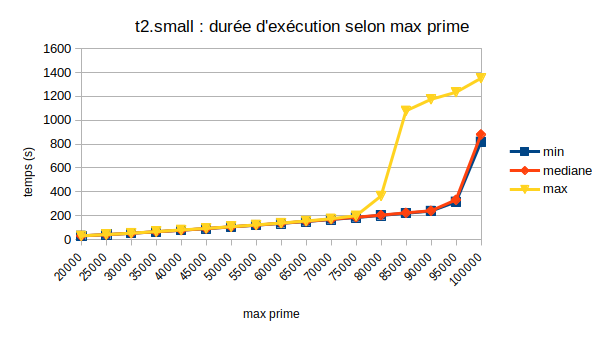
\includegraphics[width=0.9\linewidth]{images/cputSmallRaw}
\caption[t2.small sysbench]{comportement de t2.small sous sysbench}
\label{fig:cputsmallraw}
\end{figure}

On remarque la brusque montée du temps d'exécution sur la figure \ref{fig:cputsmallraw}. Cette monté s'explique par le fait que les images \textit{t2.small} ont un fonctionnement particulier: lorsqu'elles sont au repos elles emmagasinent des crédits cpu qui sont consommés lorsque le processeur est sollicité. Une fois que tous les crédits cpu sont utilisés, la performance diminue drastiquement. Ce qui se manifeste par une brusque monté du temps d'exécution. La courbe représentant le max monte plus vite car la machine associée à cette courbe à commencé avec moins de crédit cpu que les autres. Elle n'était pas assez reposée lors du test. Pour confirmer que le critère affectant les performances est bien le temps et non l'exigence du calcul, nous avons tracé une courbe où la valeur de \textit{max prime} est constante à 100 000. Valeur où on observe la brusque dégradation des performances sur \ref{fig:cputsmallraw}.

\begin{figure}
\centering
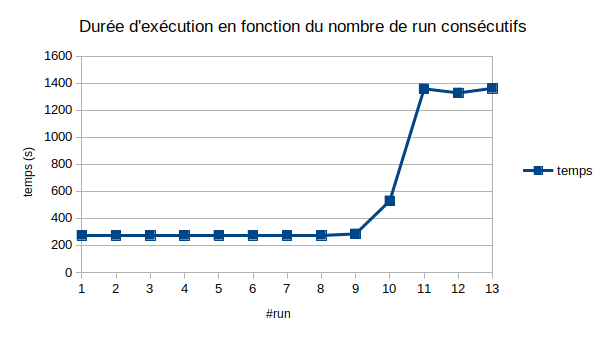
\includegraphics[width=0.9\linewidth]{images/constCpu}
\caption{Comportement de t2.small en fonction du temps de travail}
\label{fig:constcpu}
\end{figure}
Ainsi, sur la figure \ref{fig:constcpu} on peut vérifier que lorsque que la machine commence au repos, il lui faut environ 280 secondes pour compléter la tâche contre environ 800 secondes dans le cas précédent.

Les cas des instances m4.2xlarge et c4.4xlarge est plus classique
\begin{figure}
\centering
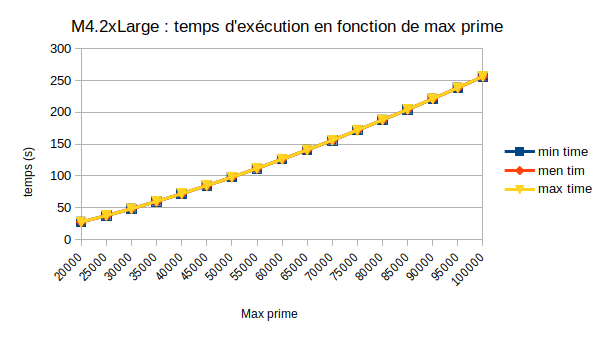
\includegraphics[width=0.9\linewidth]{images/cpuMLargeRaw}
\caption{comportement de m4.2xlarge sous sysbench}
\label{fig:cpumlargeraw}
\end{figure}
\begin{figure}
\centering
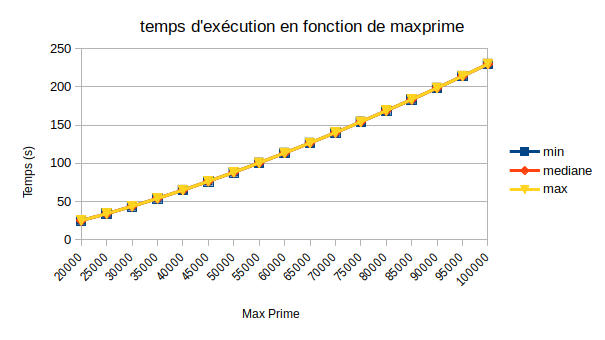
\includegraphics[width=0.9\linewidth]{images/cpuCLargeRAW}
\caption{comportement de c4.4xlarge sous sysbench}
\label{fig:cpuclargeraw}
\end{figure}

Pour ces deux instances, l'évolution de la durée est presque linéaire, ce qui, de part la nature du test, est attendue. On remarque toutefois que c4.4xlarge est globalement plus puissante que les deux autres. Enfin de faciliter la comparaison, les durées respectives pour $max prime = 100000$, sont représentées dans le tableau ci-dessus.
\newline
\begin{center}
	\begin{tabular}{|l|c|}
		\hline 
		c4.4xlarge & 230 s\\ 
		\hline 
		m4.2large & 260 s\\ 
		\hline 
		t2.small (au repos) & 280 s\\ 
		\hline 
		t2.small (ayant utilisé tous ses crédits) & 1300 s\\ 
		\hline 
	\end{tabular}
\end{center} 

Évaluons maintenant les performances de Azure. Afin que la comparaison soit possible, les mêmes tests que précédemment ont été réalisés sur les instances A1, A8 et D5.

\begin{figure}
\centering
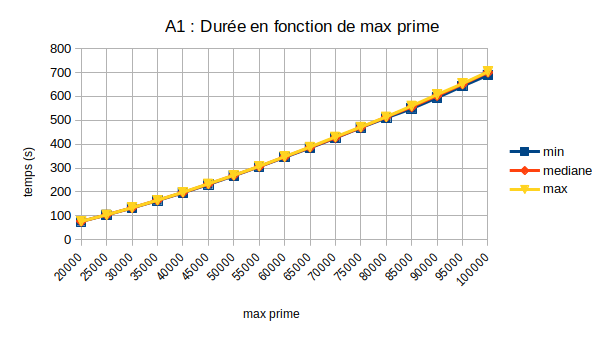
\includegraphics[width=0.9\linewidth]{images/cupA1RAW}
\caption{comportement de A1 sous benchmark}
\label{fig:cupa1raw}
\end{figure}

\begin{figure}
\centering
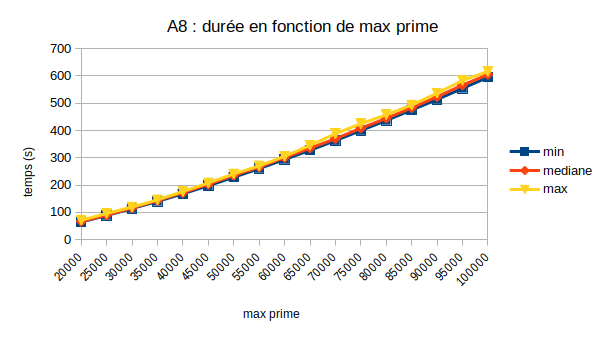
\includegraphics[width=0.9\linewidth]{images/cpuA8RAW}
\caption{comportement de A8 sous sysbench}
\label{fig:cpua8raw}
\end{figure}

\begin{figure}
\centering
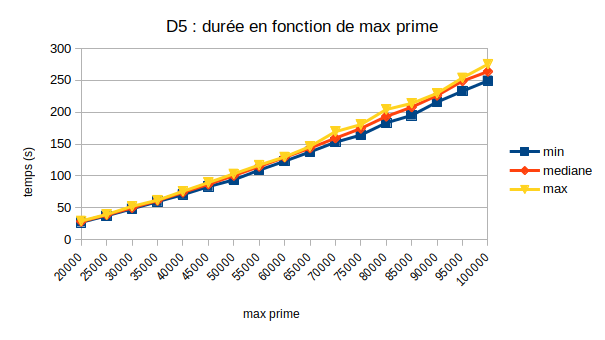
\includegraphics[width=0.9\linewidth]{images/cpuD5RAW}
\caption{comportement de D5 sous sysbench}
\label{fig:cpud5raw}
\end{figure}

Les figures  \ref{fig:cupa1raw}, \ref{fig:cpua8raw}, \ref{fig:cpud5raw} présentent des courbes dont les résultats sont nettement inférieurs à ceux des instances m4.2xlarge et c4.4xlarge.

Il résulte des résultats précédents qu'en termes de puissance
brute, l'intance cx4.2large est de loin la meilleure. Nous allons maintenant comparer leur performance respectives lorsque que l'utilisation de threads rentre en jeu. Pour cela,
nous utilisons la commande suivante:
\newline
\begin{center}
	sysbench --test=cpu --num-threads=\textbf{valeur} --cpu-max-prime=100000 run
\end{center}

Pour chaque instance, à l'exception de t2.small, on fait varier le nombre de \textit{threads} de 1 à 8 afin d'observer les effets du parallélisme sur la performance. On notera que de part les résultats précédents et la description des instances, on s'attend à ce que ce soit cx4.2large qui ait les meilleures performances. Nous avons choisi de ne pas étudier t2.small, car de part les particularités de son comportement, elle n'est pas adaptée aux applications faisant énormément de calculs. En effet, si cette instance est toujours sollicitée pour de nouveaux calculs, elle ne peut jamais se "reposer" et donc recharger ses crédits CPU. Elle serait donc prisonnière de son état le moins productif.
\begin{figure}
\centering
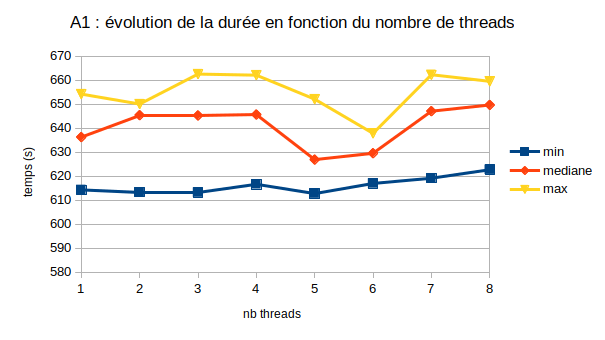
\includegraphics[width=0.9\linewidth]{images/cpuA1threads}
\caption{comportement de A1 sous sysbench en faisant varier le nombre de threads}
\label{fig:cpua1threads}
\end{figure}

\begin{figure}
\centering
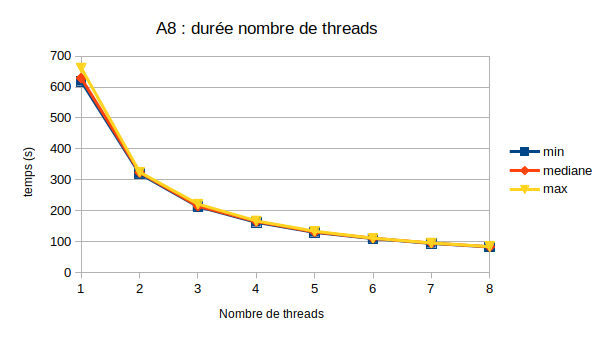
\includegraphics[width=0.9\linewidth]{images/cpuA8Threads}
\caption{comportement de A8 sous sysbench en faisant varier le nombre de threads}
\label{fig:cpua8threads}
\end{figure}

\begin{figure}
\centering
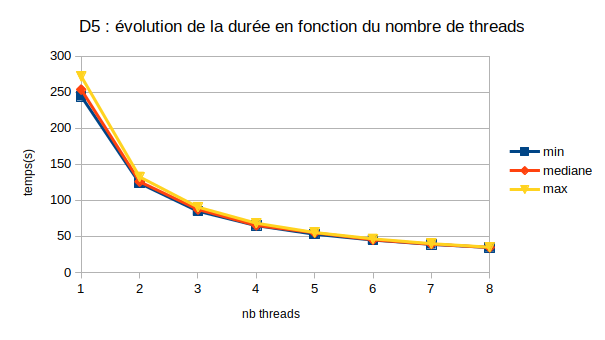
\includegraphics[width=0.9\linewidth]{images/cpuD5Threads}
\caption{comportement de D5 sous sysbench en faisant varier le nombre de threads}
\label{fig:cpud5threads}
\end{figure}

\begin{figure}
\centering
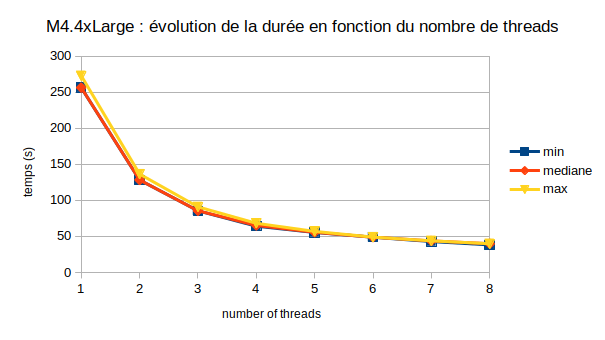
\includegraphics[width=0.9\linewidth]{images/cpuMLargeThreads}
\caption{comportement de m4.4xlarge sous sysbench en faisant varier le nombre de threads}
\label{fig:cpumlargethreads}
\end{figure}

\begin{figure}
\centering
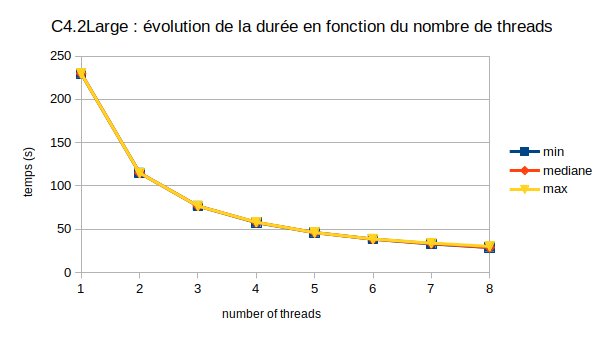
\includegraphics[width=0.9\linewidth]{images/cpuCLargeThreads}
\caption{comportement de c4.2xLarge sous sysbench en faisant varier le nombre de threads}
\label{fig:cpuclargethreads}
\end{figure}

Les résultats sur les figures \ref{fig:cpua1threads}, \ref{fig:cpua8threads}, \ref{fig:cpud5threads}, \ref{fig:cpumlargethreads} et \ref{fig:cpuclargethreads} sont conformes à l'intuition. La machine A1 n'ayant qu'un cœur ne bénéficie pas des avantages du parallélisme. Tandis que les autres machines, ayant toutes au moins 8 cœurs, voient leur performance s'améliorer. Afin d'améliorer la lisibilité nous allons résumer les différentes durée d'exécution de chaque instance pour une exécution à 8 threads. 
\begin{center}
	\begin{tabular}{|l|c|}
		\hline 
		c4.2xlarge & 28,8 s \\ 
		\hline 
		m4.4xlarge & 39,8 s \\ 
		\hline 
		A1 & 649,6 \\ 
		\hline 
		A8 & 82,9 s \\ 
		\hline 
		D5 & 34,6 s \\ 
		\hline 
	\end{tabular}
\end{center} 
Précisons que les valeurs dans le tableau correspondent à la médiane des 5 exécutions. Il en résulte que le type d'instance le plus performant en terme de cpu est c4.2xlarge.


\subsection{dd}
	Nous allons tester les opérations IO avec la commande dd.
	dd fait partie des commandes de base des Systèmes Unix. Elle permet
	de copier des sections du disque directement.
	C'est une copie brute et donc indépendante du contenu et du 
	système de fichiers. Cela nous permet donc de mesurer les capacités
	effectives du disque. On va lancer la commande: \\
	\begin{center}
		dd if=/dev/zero of=sb-io-test bs=1M count=1k conv=fdatasync
	\end{center}
	L'option count indique que l'on va copier 1000 blocs, l'option bs
	correspond à la taille du bloc. On va donc copier 1G de données brutes.
	L'option if indique depuis où nous allons copier les données, /dev/zero
	est une sorte de fichier virtuel composé uniquement de zero. On copier
	les données vers la zone désignée par l'argument of.
	Le fait d'ajouter l'option conv=fdatasync fait en sorte que la commande
	ait fini d'écrire sur le disque à l'endroit désiré avant de terminer.
	Sans cette option dd retourne après avoir passé les données à la RAM.
	C'est donc une bonne mesure qui sera proche de l'utilisation réelle.
	Nous obtenons les résultats visibles sur la figure \ref{fig:io}. On constate que globalement les machines amazon ont, et de loin, un meilleur débit. En particulier,
	les machines m4.4xlarge et c4.2xlarge ont de très bons résultats. Leur débits est presque trois fois supérieur à ceux des autres machines.
\begin{figure}
\centering
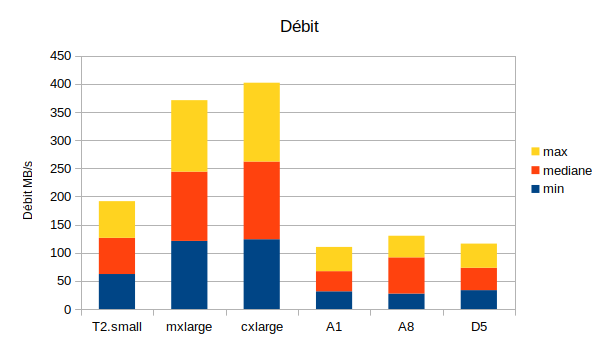
\includegraphics[width=0.9\linewidth]{images/IO}
\caption{Comparaisons des débits des différentes machines}
\label{fig:io}
\end{figure}

\pagebreak
\subsection{Bonnie++}
\subsubsection{Présentation}
	Bonnie++ est un test un peu plus avancé pour le disque.
	Bonnie fait plusieurs tests consécutivement, il permet de tester trois
	quantités:
	\begin{itemize}
	\item La vitesse de lecture et d'écriture
	\item Le nombre de seeks effectué par secondes
	\item Des opérations sur les metadata
	\end{itemize}
	Bonnie va procéder en faisant des lectures,écritures,créations et
	suppression de fichiers de façon consécutive et à la fois aléatoire.
	Ces tests permettent de bien séparer ces quantités et permet 
	d'assurer qu'une machine a bien les compétences nécessaires en
	lecture/ecriture mais aussi en gestion de fichier. Cela va être
	utile pour benchmarker une machine qui va possiblement avoir à gérer
	beaucoup de créations et de suppressions de fichiers comme un serveur
	mail.\\

\subsubsection{Benchmarking}
	Idéalement pour ne pas avoir un test biaisé par le cache, le dataset
	devrait être au moins deux fois plus grand que la taille de la RAM. Par
	défaut Bonnie utilise un dataset de deux fois la taille de la RAM. \\

	On utilise la commande:
	\begin{center}
		bonnie++ -s size -r size2 -b
	\end{center}
	Le -b indique qu'on demande que les opérations soient synchronisés,
	c'est à dire qu'on évite le buffering qui masquerait le temps réel de
	lecture/écriture et création de fichier.
	L'option -s spécifie la taille du dataset.  L'option -r spécifie la
	taille de la RAM car Bonnie n'autorise pas les exécutions avec moins que
	deux fois la RAM.

	Le problème avec les grosses instances d'Amazon est qu'elles ont très
	peu d'espace disque et une grosse RAM. Par exemple la m4 dispose de 32G
	de RAM et seulement 9G d'espace disque disponible. On va donc indiquer
	à Bonnie de n'utiliser qu'une partie de la RAM avec l'option -r et
	utiliser une taille de dataset inférieure à 9G, soit 8G. Il semble
	cependant que malgré l'option -r le programme utilise toute la RAM car
	en essayant avec deux tailles de RAM différentes (5G et 55G sur Azure)
	et sans synchronisation (afin que la RAM ait un impact) les temps
	étaient très proches. On ne peut donc pas contrôler la RAM utilisée par
	Bonnie.

	Pour l'instance t2.small d'Amazon et l'instance A1 d'Azure qui ont plus
	de deux fois leurs RAM en espace disque on appellera bonnie++ seulement
	avec l'option -b.
	\begin{center}
		bonnie++ -b
	\end{center}
	On aura un dataset de 4G avec 2G de RAM.
	Pour les instances ayant un disque de taille assez inférieure à deux fois leur RAM,
	soient les autres instances, on va utiliser un dataset plus petit.
	Pour les instances Amazon (m4.2xlarge et C4.4xlarge) qui ont moins de mémoire:
	\begin{center}
		bonnie++ -s 8000 -r 4000 -b
	\end{center}
	Soit un dataset de 8G et l'option -r est là seulement pour forcer Bonnie à s'exécuter.
	Enfin pour les autres instances Azure(A8\_v2 et D5\_v2):
	\begin{center}
		sudo bonnie++ -d /mnt/ -b -u root
	\end{center}

	Les tests ne sont donc pas très équitables car certaines machines vont
	profiter de leur RAM. Mais cela reflète l'utilisation réelle et
	l'option -b essaye de minimiser cet avantage. \\

	Nous comparons maintenant les différentes machines sur les trois 
	caractéristiques que mesure Bonnie. Nous traçons trois barplots
	différents correspondant à chaque groupe de tests.
	Les noms des tests sont en abscisse et il y a une barre contenant
	chaque mesure pour chaque machine, on a donc 6 barres pour chaque 
	teste. Entre parenthèse est l'unité de mesure du temps, en 
	millisecondes (MS) ou microsecondes (us). En ordonnée est la valeur
	correspondante. \\
	\begin{figure}[htbp]
	\begin{center}
	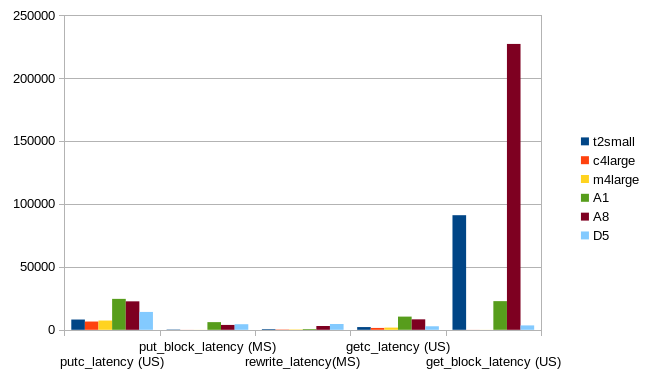
\includegraphics[scale=0.9]{images/readwrite.png} 
	\caption{Opérations de lecture/ecriture sequentielle et random}
	\label{fig:fig0}
	\end{center}
	\end{figure}
	\begin{figure}[htbp]
	\begin{center}
	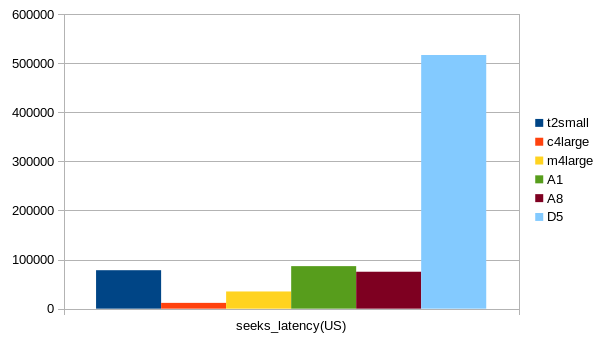
\includegraphics[scale=0.9]{images/seek.png} 
	\caption{Seeks}
	\label{fig:fig0}
	\end{center}
	\end{figure}
	\begin{figure}[htbp]
	\begin{center}
	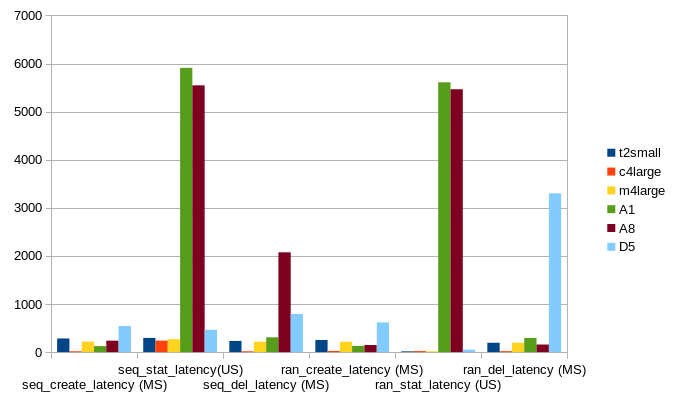
\includegraphics[scale=0.9]{images/metadata.png} 
	\caption{Opération sur les fichiers et les metadata}
	\label{fig:fig0}
	\end{center}
	\end{figure}

	Pour les tests de lectures/écritures les machines Amazon sont en général
	très bonnes et meilleures que les machines Azure qui semblent se valoir.
	La machine t2.small a cependant une grosse latence inexpliquée sur le 
	dernier test ce qui limite la confiance que l'on peut avoir dans cette
	instance qui n'est pas très fiable sur les lecture de blocs, 
	possiblement à cause de sa RAM limitée.
	Les machines Azure ont des comportements similaires entre elles mais
	D5 semblent être globalement plutôt meilleure. On note que 18 a eue
	aussi une très grosse latence lors de la lecture par blocs. \\

	Pour les tests de seek la meilleure machine est la c4large de loin et
	la pire de loin est la d5 d'Azure. En moyenne cette dernière était
	correcte mais elle a eu un pic de latence. \\

	Pour les opérations sur les fichiers, là encore les machines Amazon sont
	bien meilleures. La A1 et la A8 d'Azure étant particulièrement très
	mauvaise et de façon consistante. \\

\pagebreak
\subsection{Stress-ng}
\subsubsection{Présentation}
	Nous allons utiliser l'outil stress-ng afin de tester la mémoire des
	instances. Stress-ng peut stresser aussi d'autres quantités mais nous
	allons nous concentrer sur la mémoire.\\
	Stress-ng permet de stresser le système, c'est à dire qu'il cherche
	à pousser le système à des cas d'utilisations extrêmes afin de voir 
	comment celui-ci va réagir. Dans le cas de la mémoire cela prend
	la forme de processus qui vont consommer beaucoup de mémoire de
	façon agressive. Ce type de test est bon car il permet de voir
	comment l'instance réagirait face à une grosse charge de travail.
	Il permet aussi de départager les instances en terme d'efficacité
	de la mémoire. On va voir si la machine D5\_v2 qui a beaucoup
	plus de RAM performe bien mieux que les autres ou non.

\subsubsection{Benchmarking}
	L'outil contient des classes qui regroupent les tests permettant de
	tester la quantité correspondante. Il y a les classes cpu, cpu-cache,
	device, io, interrupt, filesystem, memory, network, os, pipe, scheduler
	et vm.

	La classe memory comporte notamment les tests suivants:
	1 bsearch, 1 context, 1 heapsort, 1 hsearch, 1 lockbus, 1 lsearch, 1
	malloc, 1 matrix, 1 membarrier, 1 memcpy, 1 memfd, 1 mergesort, 1
	mincore, 1 null, 1 numa, 1 oom-pipe, 1 pipe, 1 qsort, 1
	remap-file-pages, 1 stack, 1 str, 1 stream, 1 tsearch, 1 vm, 1 vm-rw, 1
	wcs, 1 zero, 1 zlib.

	Nous pouvons spécifier le nombre de stresseur, s'ils sont exécutés de façon
	parallèle ou alors de façon séquentielle.
	Nous pouvons fixer un temps de stress.
	Nous pouvons afficher les métriques avec l'option --metrics ou 
	--metrics-brief. Un indicateur grossier de la performance est le bogo par 
	seconde (bogus operation). Cependant selon les tests la taille du bogus
	est différente et donc non comparable. \\
	L'option --agressive peut être ajoutée pour ajouter plus de stimulis.
	On peut aussi lancer la commande en root afin que stress-ng contrôle
	son scheduling et donc puisse s'arranger pour challenger le système 
	encore plus.

	Pour lancer n stress de mémoire en parallèle pendant un temps t nous 
	utilisons la commande:
	\begin{center}
		stress-ng --class memory --all n -t t --metrics-brief
	\end{center}
	Cependant il y a beaucoup de test et on peut en choisir 3 pour se concentrer
	sur eux:
	\begin{itemize}
		\item brk: Augmente la taille du data segment une page à la fois,
			ajoutant donc de la mémoire au processus.
		\item stack: lance des processus faisant des \textit{stacks overflows}.
		\item bigheap: lance des processus qui augmente leur heap en
			reallouant leur mémoire.
	\end{itemize}
	Ces trois tests vont être efficaces pour tester la gestion de la mémoire.
	Afin d'avoir un stress efficace nous allons lancer 10 stresseurs pour
	chaque test en parallèle, en root et en rajoutant l'option --aggressive.
	Soit la commande:
	\begin{center}
		sudo stress-ng --brk 10 --stack 10 --bigheap 10 --metrics-brief --aggressive -t 30
	\end{center}

	Nous obtenons les résultats reportés sur les graphiques suivants. Un
	plus grand nombre de bogo op/s indique une meilleure performance. Ce n'est pas
	une mesure exacte mais cela permet d'avoir un aperçu.\\
	La hiérarchie semble bien respectée sur les deux premiers tests (brk et bigheap),
	on peut voir que t2small et A1 sont du même ordre de grandeur, m4large et A8 aussi.
	Cependant la machine D5 écrase toutes les autres, montrant la puissance de sa mémoire
	et notamment de ses 55G de RAM. \\
	Le dernier test vient confirmer cette hegemonie, les autres machines ayant toutes assez 
	mal performé, cela étant dû au fait qu'il y avait déjà deux gros tests qui roulaient.
	Mais cela a permis de pousser les machines à leurs limites, on voit étonnamment que A1
	a bien performé sur ce test là.

	\begin{figure}[htbp]
	\begin{center}
	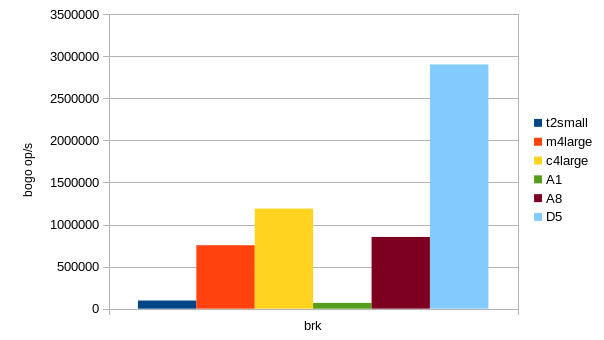
\includegraphics[scale=0.9]{images/brk.png} 
	\caption{Comparaison des performances sur le test brk}
	\label{fig:fig0}
	\end{center}
	\end{figure}
	\begin{figure}[htbp]
	\begin{center}
	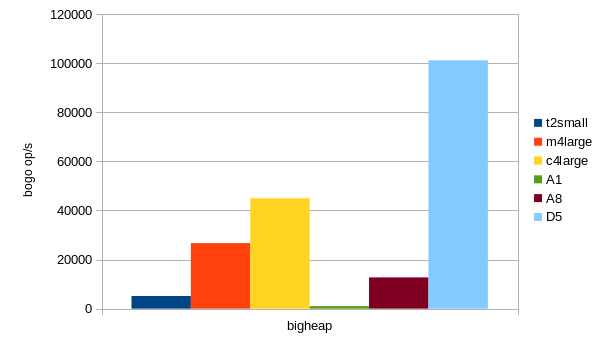
\includegraphics[scale=0.9]{images/bigheap.png} 
	\caption{Comparaison des performances sur le test bigheap}
	\label{fig:fig0}
	\end{center}
	\end{figure}
	\begin{figure}[htbp]
	\begin{center}
	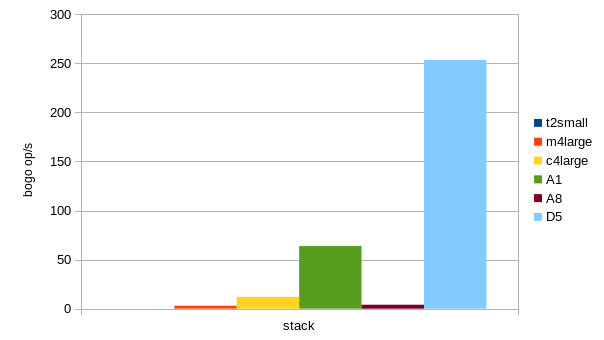
\includegraphics[scale=0.9]{images/stack.png} 
	\caption{Comparaison des performances sur le test stack}
	\label{fig:fig0}
	\end{center}
	\end{figure}

\pagebreak
\subsection{hdparm}
\subsubsection{Présentation}
%Hdparm is a benchmark to set and view disk parameters as well as testing reading speeds. For this work, it will be used to analyze the disk performance by evaluating and comparing the disk and cache reading speed. The output is basically an indication of the throughput of the processor, cache and memory.
%Hdparm is easy to use and provides meaningful data for the analysis of the different instances.

%We use Hdparm to perform the timings of device reads for benchmark and comparison purposes. Moreover, this operation should be repeated 2 at 3 times on an inactive system. This displays the speed of reading through the buffer cache to the disk without any prior caching of data.  %

%This measurement is an indication of how fast the drive can sustain  sequential
%data reads under Linux, without any filesystem overhead. To ensure accurate
%measurements, the buffer cache is flushed during the processing of -t using the BLKFLSBUF ioctl.%
Hdparm est une référence pour définir et afficher les paramètres du disque ainsi que pour tester
la vitesse de lecture. Pour ce travail, il sera utilisé pour analyser les performances du disque et du cache lors d'une lecture. Le résultat de la commande est
essentiellement une indication du débit du processeur, du cache et de la mémoire.
Hdparm est facile à utiliser et fournit des données significatives pour l'analyse des 
différentes instances.

Nous utilisons Hdparm pour effectuer les chronométrages des lectures de périphériques. Cette opération doit être répétée 2 à 3 fois
sur un système inactif. Ceci affichera la vitesse de lecture à travers le tampon
Cache sur le disque sans qu'aucune mise en cache préalable des données n'est été faite.

Cette mesure permet de visualiser à quelle vitesse les lectures depuis le disque peuvent être faites,sans les délais dus au système de fichiers. Afin de garantir la validité des mesures, le cache est vidé grâce à l'option -t.
BLKFLSBUF ioctl.
\subsubsection{Benchmarking}
%After making the hdparm benchmark ten times of the instances in azure and amazon, we collect our results and we take the median of benchmarking from each instance. Besides, we plot the results on the following chart to show the capacities of each instance and to figure which virtual machine has the best time reading from the disk (in  MB / sec).

%We notice in the following chart of the performance of reading from disk is different between instances. It is clear that both instances of type C4.4Xlarge and M4.2Xlarge have the best time of disk read capacities With 170 MB/s as approximate values.

%Consequently, for this reason if we have a constraint of a lot of data traffic exchange with disk and a high capacity of reading from disk, we should choose these two instances.  

Après avoir fait le benchmark hdparm dix fois sur les instances d'azur et amazon, nous recueillons nos résultats et nous prenons la médiane de l'analyse comparative de chaque instance. En outre, nous traçons les résultats sur le graphique suivant pour montrer les capacités de chaque instance et pour déterminer quelle machine virtuelle a le meilleur temps de lecture à partir du disque (en MB / s).

Nous remarquons que dans le tableau suivant représentant, la performance des lectures à partir du disque est différente pour chaque instance. Il est clair que les deux instances de type C4.4Xlarge et M4.2Xlarge ont le meilleur temps de lecture de disque (environ 170 Mo / s).

Pour cette raison, si sous la contrainte de beaucoup d'échange de données, de trafic, avec le disque et le besoin d'une grande capacité de lecture à partir de disque, nous devons choisir une de ces deux instances.
~\\
\centerline{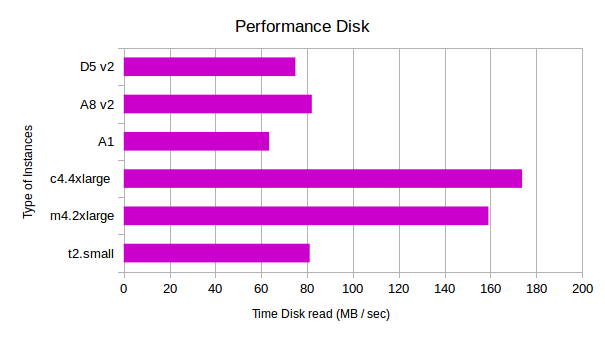
\includegraphics[width=0.95\textwidth]{images/disk.png}} % Include the image placeholder.png
\centerline{Figure : Performance de lecture du Disque} 
~\\

\pagebreak
\subsection{SpeedTest}
\subsubsection{Présentation}
%We use Speedtest to perform the internet connection speed. It is a script written in Python which measures the internet speed bidirectionally. This application allows us to check the internet speed upon distance in km, we can test it against specific servers and it also provides a URL so that you can share your result on the internet.  After executing the Speedtest application, it test your broadband connection by downloading a file from a nearby speedtest.net server on the web. It returns the results of speed of Download and Upload in Mbit/s. Consequently, we could identify the performance of the connection of each instances.
Nous utilisons \textit{Speedtest} pour mesurer la vitesse de connexion Internet. C'est un script écrit en Python qui mesure la vitesse d'Internet de façon bi-directionnelle. Cette application nous permet de vérifier la vitesse d'Internet sur la distance en km, nous pouvons le tester contre des serveurs spécifiques et il fournit également une URL afin que vous puissiez partager votre résultat sur l'Internet. Après l'exécution de l'application \textit{Speedtest}, il teste votre connexion haut débit en téléchargeant un fichier d'un serveur \textit{speedtest.net} à proximité sur le Web. Il renvoie les résultats de la vitesse de téléchargement et de téléversement en Mbit / s. Par conséquent, nous pouvons mesurer la connexion de chaque instance.

\subsubsection{Benchmarking}
De nos jours, il est très important pour les petites et les grandes entreprises d'être en ligne tout le temps. Il est nécessaire de vérifier la vitesse de connexion Internet pour assurer une bonne connexion pour nos besoins. Pour cette raison et pour identifier lesquelles des machines virtuelles que nous étudions ont une meilleure connexion Internet, nous avons réalisé un benchmark en utilisant la bibliothèque speedtest.

Pour chaque machine, nous avons effectué le test 10 fois et nous avons pris la médiane des résultats. Dans les deux graphiques suivants, nous avons collecté les résultats médians de téléchargement et de téléversement pour chaque instance.

Dans le graphe de téléversement, nous constatons une différence faible entre les différentes machines avec des valeurs allant de 150 Mbit / s pour la C4.4Xlarge machine à 280 Mbit / s pour la machine D5-v2. Pour cette raison, nous n'allons pas mettre une grande importance à comparer entre la machine virtuelle basée sur la capacité de téléversement.

Pour le graphique de téléchargement, nous notons que nous avons deux machines A8-v2 et D5-v2 ont une capacité de téléchargement estimée à 1750 Mbit / s. Pour cette raison, si nous avons la nécessité d'un bon débit ascendant, nous choisirons une de ces machines.
%Nowadays, it is highly important for businesses and big companies to be online all the time.  It is necessary to check internet connection speed to ensure a good connection for our need. For this reason and to identify which virtual machines we are studying have better internet connection, we have realized a benchmark using the The speedtest library.

%For each machine, we performed the test 10 times and we took the median of results. In the following two chart we have collected the median results of download and upload for each instance.

%In the upload chart, we notice a simple difference between the different machines with values ranging from 150 Mbit/s for the C4.4Xlarge machine to 280 Mbit/s for the D5-v2 machine. For this reason we are not going to put great importance to compare between the virtual machine based on the ability of upload. 

%For the Download chart, we note that we have two machines A8-v2 and D5-v2 have a significant download capacity which is estimated to be 1750 Mbit/s. For this reason, if we have a constraint of need for a high internet connection we will Choose these two machines A8-v2 and D5-v2.
~\\
\centerline{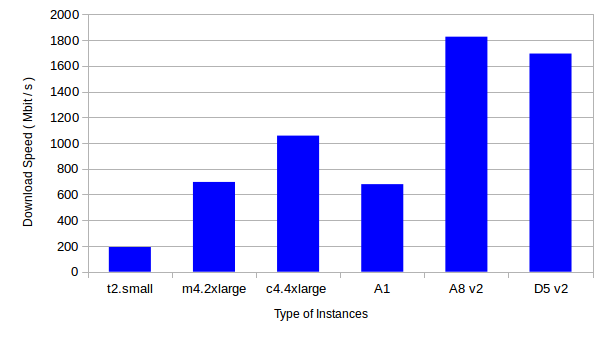
\includegraphics[width=0.95\textwidth]{images/download.png}} % Include the image placeholder.png
\centerline{Figure : débit descendant} 
~\\

~\\
\centerline{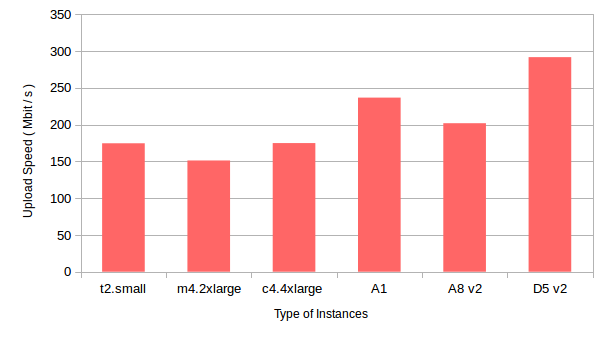
\includegraphics[width=0.95\textwidth]{images/upload.png}} % Include the image placeholder.png
\centerline{Figure : débit ascendant} 
~\\

\pagebreak
\section{Problem}

Après avoir jauger les différentes instances nous sommes plus à même 
de décider d'une solution pour l'entreprise Alpha X. \\
Cette entreprise a plusieurs besoins différents:
\begin{itemize}
	\item Stockage: il y a un besoin de stocker les données historiques.
		Nous n'avons pas d'informations sur la quantité de données, 
		celle-ci va surement être importante car de gros calculs
		vont être fait dessus. Il se peut aussi que les données 
		arrivent en temps réel il faudrait donc un stockage de données
		elastique au cas où. Une instance Amazon rattachée à EBS
		sera une bonne solution. Il nous faut aussi un système
		rapide en lecture/écriture disque et en gestions des
		fichiers. \\
		Une des meilleures instances pour ce travail était la
		c4.4xlarge d'Amazon. Nous avons observé cela lors des
		tests dd, Bonnie++ ou encore hdparm.\\
		Il faut toutefois une vitesse correcte en upload pour
		transmettre les données à la VM2 ce qui est le cas
		de c4.4Xlarge. Alors nous admettons l'instance c4.4Xlarge dans la VM1.
	\item Business Intelligent Services: Nous avons besoin ici
		d'instances étant capable de réaliser du calcul
		haute performance en parallèle. Le master pourrait
		être une instance un peu moins puissante puisqu'elle
		aura plus un rôle de contrôle et de rassemblement
		des résultats. De ce fait, on optera sûrement pour une machine m4.4xlarge ou c4.2xlarge selon le budget disponible. Ensuite, selon le rôle que l'on attribue au master (simple répartiteur de charge? prend part aux calculs?). On peut donc imaginer un master de type
		m4.4xlarge et des slaves de type c4.2xlarge. Cette configuration aurait pour but de diminuer les coûts la m4.4xlarge étant moins onéreuse que c4.2xlarge.
	\item Data extraction: Les meilleures types d'instances en termes d'IO et d'IOPS sont m4.4xlarge et c4.2xlarge.
	Une fois encore, il serait donc pertinent de choisir une de ces deux instances. \'A moins que la différence de performances justifie réellement l'investissement, la m4.4xlarge devrait convenir et être moins chères que la c4.2xlarge. Toutefois, dans la situation hypothétique d'un budjet infini, nous choisirions cette dernière car plus performante.
\end{itemize}

\section{Paper}
\begin{itemize}
	\item 1) Cette question est traitée à la section 2.
	\item 2) On a répondu à cette question dans chaque section de référence
	\item 3) Le problème principal auquel nous nous sommes heurtés est l'utilisation d'un compte gratuit. En effet, cela limite les possibilités de création de VM et donc ralentit l'obtention des résultats. Ainsi, sous Azure, on ne peut utiliser plus de 20 cpu en même temps. De même, sous Amazon on ne peut pas créer simultanément plusieurs instances des types les plus onéreux. Et on est également limité sur le nombre de VM que l'ont peut créer en série. De plus, certains tests (sysbench notamment) mettaient plus de 3h à compléter. Les répéter 5 fois pour chaque instance est donc fondamentalement long. Cela est d'autant plus vrai que pour l'instance t2.small, il fallait attendre plusieurs heures entre chaque exécution pour que le crédit cpu se recharge. Sous peine de quoi les résultats n'étaient pas comparables.
	
	Toutefois, l'utilisation du script \textit{bench.sh} en conjonction avec les outils usuels du bash (alert, script) permettait une bonne automatisation des tâches.
	\item 4) Voir les sections relatives aux tests spécifiques.
En général, nous avons été impressionnés par la cohérence
La technologie. Par exemple, avec dd, nous avons eu une variabilité très faible
Même entre le membre du groupe qui se trouve sur le même
Type d'instance. Nous avons encore rencontré des résultats surprenants
Et une certaine variabilité sur d'autres tests, mais il a été isolé.
	\item 5) Voir la section Problème.
\end{itemize}

\section{Références:}
% https://doc.ubuntu-fr.org/dd
% https://romanrm.net/dd-benchmark
\subsection{Bonnie++:}
\begin{itemize}
	\item Manuel de Bonnie++
	\item https://blogs.oracle.com/roch/entry/decoding\_bonnie
	\item https://www.linux.com/news/using-bonnie-filesystem-performance-benchmarking
	\item https://www.jamescoyle.net/how-to/599-benchmark-disk-io-with-dd-and-bonnie
\end{itemize}
\subsection{Stress-ng}
\begin{itemize}
	\item Manuel de stress-ng 
	\item https://wiki.ubuntu.com/Kernel/Reference/stress-ng
	\item https://openbenchmarking.org/showdown/pts/stress-ng
	\item https://www.cyberciti.biz/faq/stress-test-linux-unix-server-with-stress-ng/
\end{itemize}
\subsection{Hdparm}
\begin{itemize}
\item Manual of Hdparm
\item https://en.wikipedia.org/wiki/Hdparm
\item http://unix.stackexchange.com/questions/108838/how-can-i-benchmark-my-hdd
\end{itemize}
\subsection{Speedtest}
\begin{itemize}
\item Manual of speedtest 
\item https://www.howtoforge.com/tutorial/check-internet-speed-with-speedtest-cli-on-ubuntu/
\item https://en.wikipedia.org/wiki/Speedtest.net
\end{itemize}
\subsection{sysbench}
\begin{itemize}
\item https://www.howtoforge.com/how-to-benchmark-your-system-cpu-file-io-mysql-with-sysbench

\end{itemize}


\end{document}
